\section{Технический проект}
\subsection{Общая характеристика организации решения задачи}

Необходимо спроектировать и разработать программную систему, которая должна способствовать сокращению исходного кода программ без ущерба их функциональности за счёт возможностей метапрограммирования.

Для достижения этой цели было принято решение спроектировать язык программирования и создать программу для его интерпретации, удовлетворяющие описанным выше требованиям.

Главной задачей разработки интерпретатора языка программирования является создание программного обеспечения, которое способно интерпретировать и выполнить исходный программный код, написанный на определенном языке программирования, так, что результат выполнения соответствует правилам, описанным в спецификации интерпретируемого языка.

Для обеспечения конкурентноспособности интерпретатора, эта задача должна выполняться как можно более эффективно и быстро. Кроме того, он должен выполнять свою задачу в соответствии с главным принципом интерпретации -- код программы обрабатывается по одной инструкции или группе инструкций, выполняющихся сразу после анализа и обработки. 

Для реализации интерпретатора необходимо разработать следующие компоненты: лексический анализатор, синтаксический анализатор, инструментарий выполнения команд языка и сборщик мусора.

\subsection{Обоснование выбора технологии проектирования}

Уже многие годы сфера ИТ предоставляет массу инструментов для разработки системного ПО, коим и является разработка интерпретатора.

\subsubsection{Описание используемых технологий и языков программирования}

В процессе разработки интерпретатора ДЯП используются язык программирования C и программные средства операционной системы семейства GNU/Linux. Используемые для создания программно-информационной системы средства отвечают современным практикам разработки и являются подходящими и достаточными для решения задач, выявленных при анализе предметной области.

\subsubsection{Язык программирования C}

Низкоуровневый язык программирования C (Си) -- один из первых языков программирования и, одновременно с этим, один из самых используемых до сих пор. Его появлению в начале 1970-х годов мир обязан инженеру Деннису Ритчи из американской компании Bell Labs, разрабатывавшим его как развитие языка Би для написания операционной системы Unix. С тех пор Си стал одним из самых популярных языков для системного программирования.

Об успешности решений, принятых при его разработке, говорит впечатлительный список узнаваемых последователей, перенявших многие его идеи -- C++, C\#, Objective-C, Java, Python, PHP и другие обязаны Си своей структурой кода и базовым синтаксисом.

Узнаваемость и простота его синтаксиса, близость к аппаратной части ЭВМ, наличие компилятора почти для всех вычислительных устройств и операционных систем, обширная стандартная библиотека, а также ручное управление памятью убеждают в выборе языка С для системного программирования, коей и является разработка интерпретатора.

Ввиду того, что реализация стандартной библиотеки этого языка, libc, отличается для различных операционных систем, было принято решение выбрать целевой платформой для разработки интерпретатора одно семейство ОС -- GNU/Linux. В этих системах применяется реализация "GNU C Library" (glibc).


\subsection{Компоненты интерпретатора}

\begin{figure}[ht]
	\center{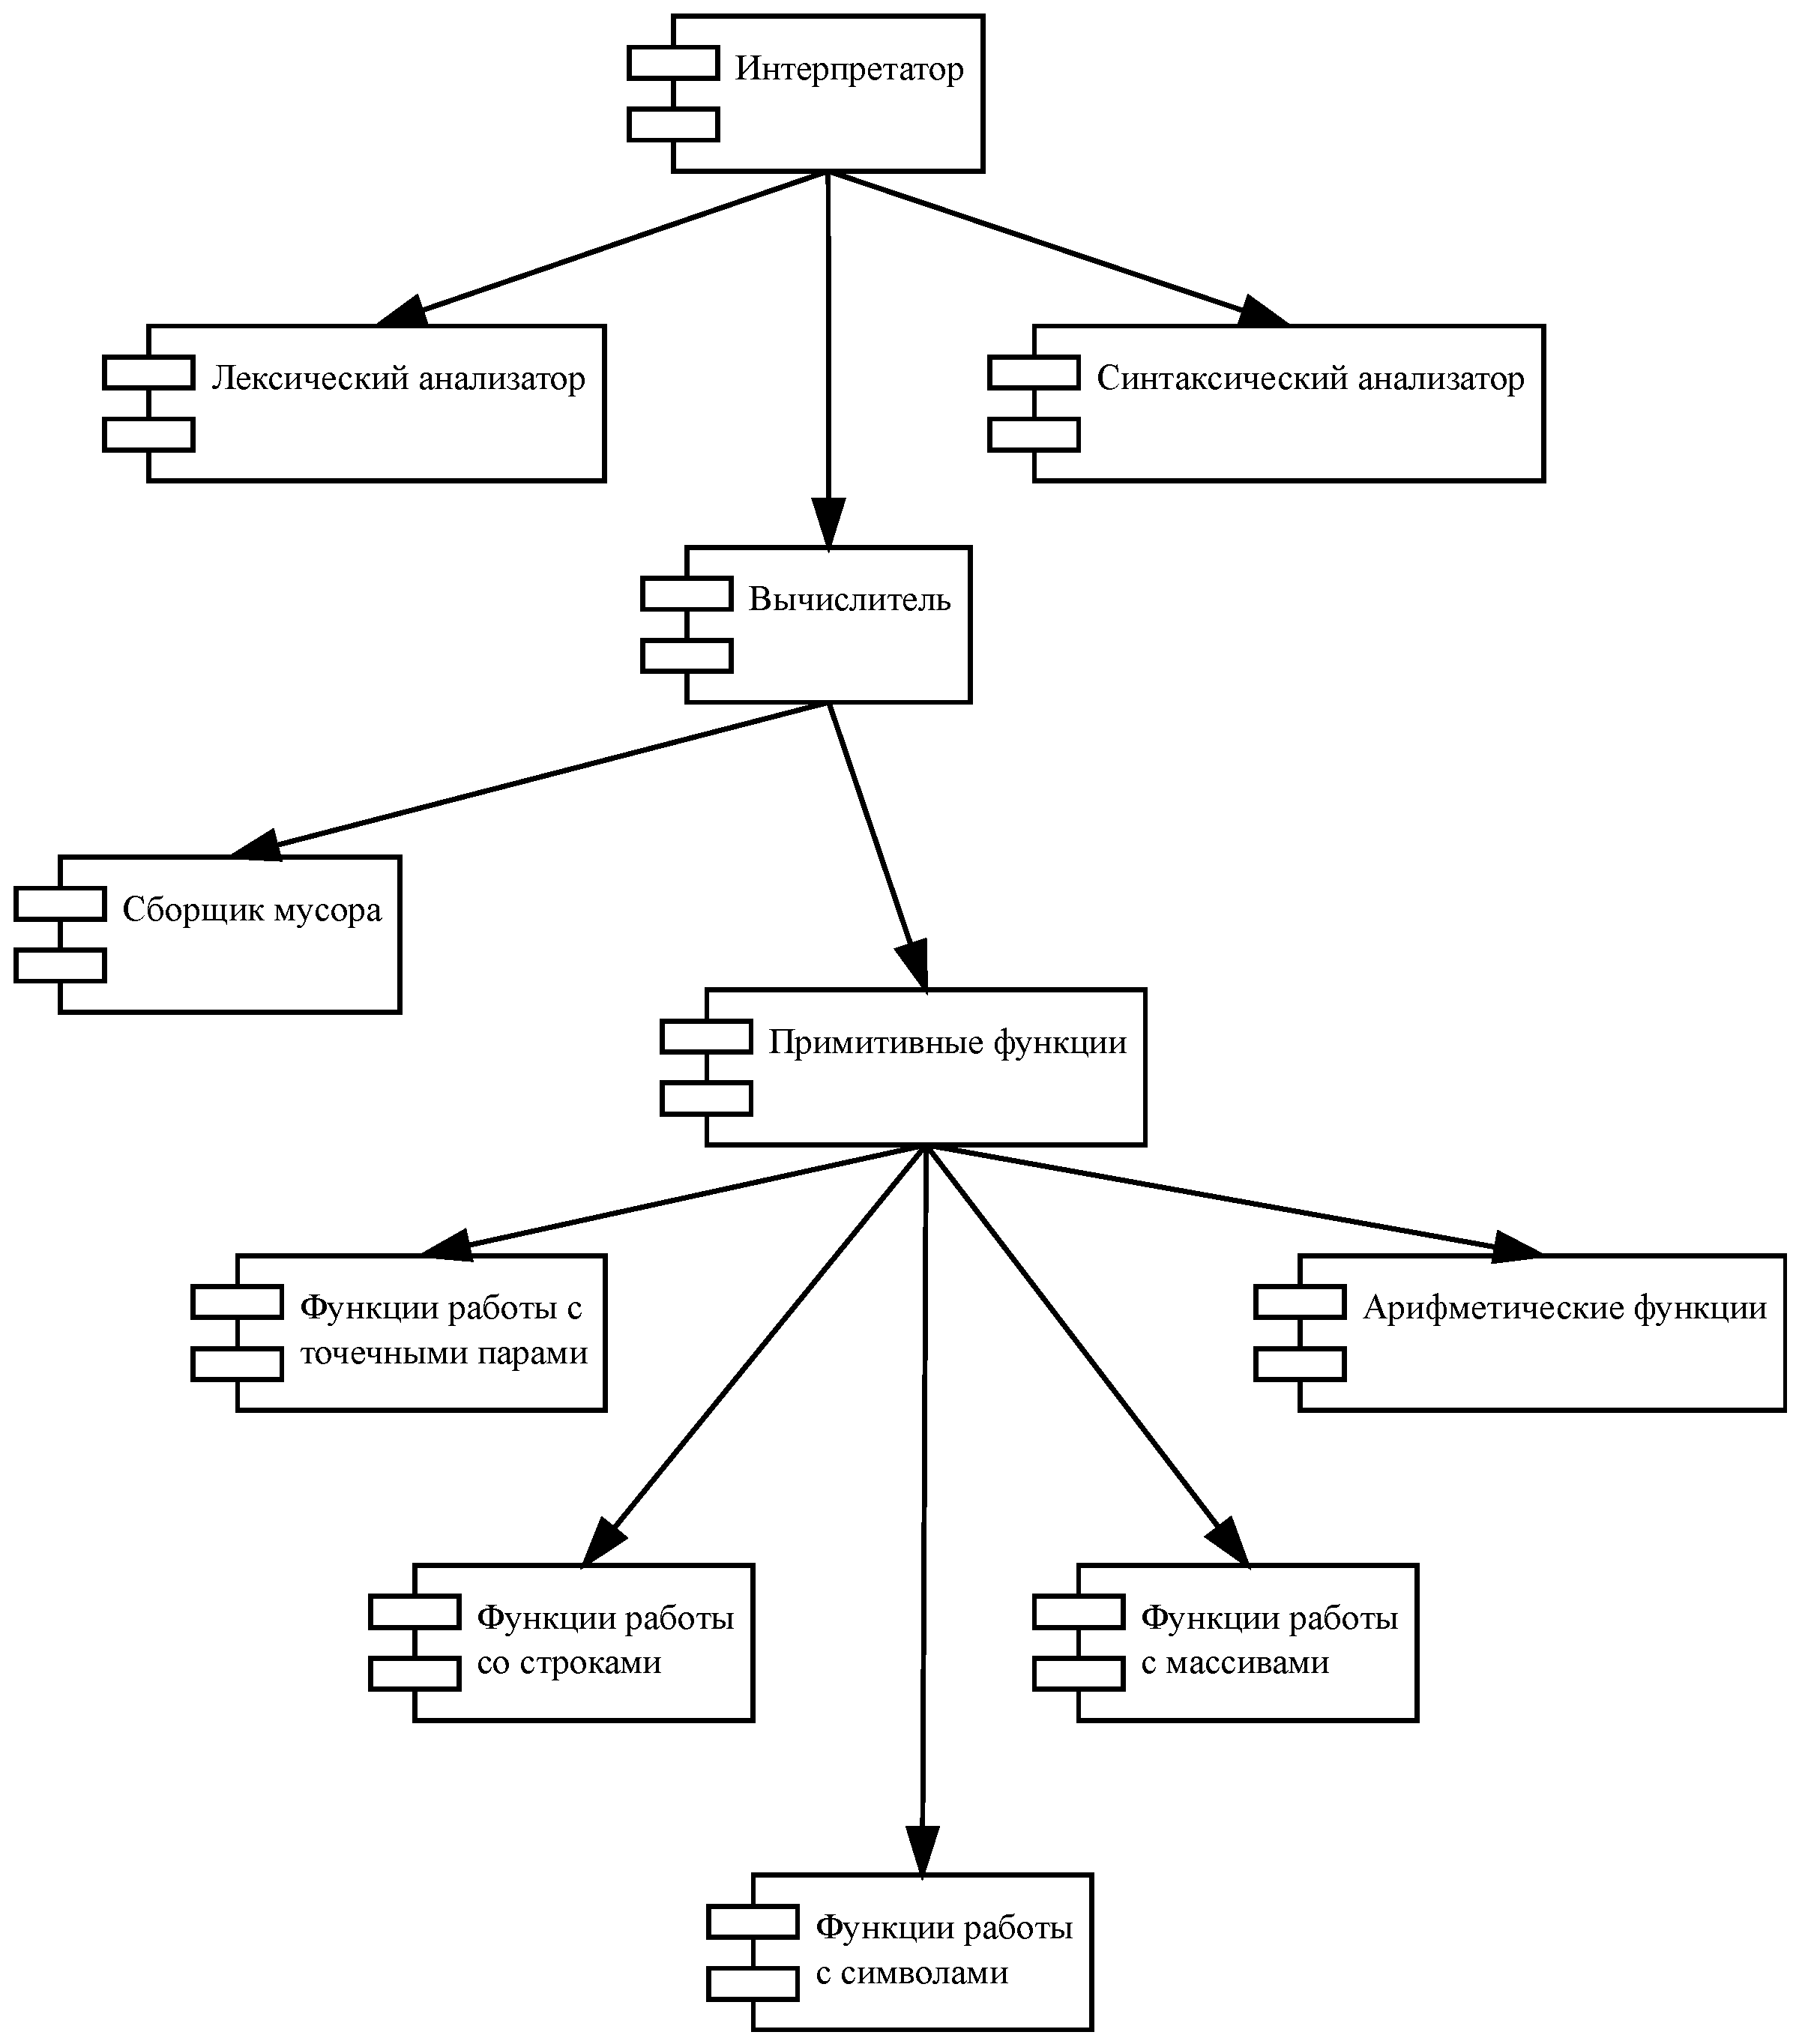
\includegraphics[width=1\linewidth]{kompdiagram}}
	\caption{Диаграмма компонентов интерпретатора}
	\label{kompdiagram:image}
\end{figure}

На рисунке \ref{kompdiagram:image} в виде UML-диаграммы показаны компоненты, составляющие интерпретатор.



\subsubsection{Алгоритм взаимодействия компонентов}
Пошаговый алгоритм взаимодействия компонентов, составляющих интерпретатор:

Шаг 1. Инициализируем исполнитель и регистрируем все примитивные функции ДЯП;

Шаг 2. Сохраняем текущее состояние программы, сохранив регистры процессора и стек с помощью setjmp. Если во время работы интерпретатора произойдёт ошибка -- вывести на экран сообщение об ошибке и перейти к шагу 8;

Шаг 3. Запускаем синтаксический анализатор;

Шаг 4. Синтаксический анализатор вызывает лексический анализатор;

Шаг 5. Лексический анализатор на основе символов из входного потока формирует лексему и возвращает её;

Шаг 6. Синтаксический анализатор на основе полученной лексемы формирует объект для внутреннего представления и возвращает его;

Шаг 7. Если был достигнут конец входного потока -- переходим к следующему шагу, иначе к шагу 12;

Шаг 8. Восстановить состояние программы к тому, что было сохранено на шаге 2, и перейти к шагу 13;

Шаг 9. Исполнитель производит вычисления с объектом, сформированным СА, в качестве аргумента и возвращает результат вычислений в виде объекта;

Шаг 10. Вывести возвращённый исполнителем объект на экран;

Шаг 11. Перейти к шагу 2;

Шаг 12. Сборщик мусора освобождает неиспользуемые объекты внутреннего представления. Перейти к шагу 2;

Шаг 13. Завершить работу интерпретатора.

\subsubsection{Лексический анализатор}
В разработанной программной системе лексический анализатор представляет собой компонент, в задачи которого входит считывание лексемы, проверка её на соответствие алфавиту языка и формирование токена.

Как только лексема была считана, она помещается в буфер размерностью в восемь символов.

Считанная лексема сравнивается со множеством зарезервированных под конструкции языка символов. При совпадении с каким-либо, формируется токен и ЛА возвращает его.


Сформированный токен представляет собой структуру с такими полями:
\begin{enumerate}
	\item type -- тип токена;
	\item value -- поле для токенов числового типа, содержит значение числа;
	\item str -- поле для токенов строкового типа, значение строки.
\end{enumerate}

Особым случаем является считывание строки. Как только обнаруживается символ кавычки, запускается функция, собирающая символы до тех пор, пока:
\begin{itemize}
	\item не встретит второй символ кавычки, чем будет закончено считывание строки, после чего ЛА вернёт сформированный токен;
	\item количество символов не превысит допустимую длину строки, что приведёт к ошибке;
	\item не будет достигнут конец входного потока, что также приведёт к ошибке.
\end{itemize}


Если символ не является одним из зарезервированных, производится проверка на то, является он числом или символом.

Ввиду того, что имя символа, как и отрицательное число, может начинаться со знака минус решается неоднозначность, связанная с восприятием лексическим анализатором следующих символов. Для этого считывается ещё один символ и, если он является числовым, дальнейшая запись определяется как число, иначе как символ.

Если имя символа состоит из допустимых знаков, то бишь из алфавита языка, формируется токен типа символ и возвращается как результат работы ЛА. В противном случае, выдаётся ошибка о некорректности символа.

\subsubsection{Синтаксический анализатор}
Синтаксический анализатор запрашивает у ЛА по одному токену, строит для них внутреннее представление и повторяет процесс, пока не будет сформировано одно s-выражение, затем происходит возврат выражения.

СА, как и ЛА, выполняет проверку на ошибки, но уже синтаксические. Он выявляет отсутствие аргументов у операторов цитирования и квазицитирования, неоконченность списков (отсутствие закрывающей скобки) и отсутствие списка после символа '\#' для создания массива.


\subsubsection{Объекты внутреннего представления}
Как уже было рассмотрено ранее, весь программный код, считываемый из потока ввода, ещё на этапе обработки лексическим анализатором преобразуется в особые структуры, а не хранится в виде текста, ввиду необходимости манипулирования предоставленной им информацией, что было бы проблематичным и неэффективным при текстовом хранении. После обработки синтаксическим анализатором, все данные, полученные из программного кода, принимают своё окончательное представление и при исполнении инструкций меняется уже не их представление, а содержимое.

В разрабатываемом интерпретаторе все данные хранятся в виде структур языка C. Всего было разработано пять структур. Структура верхнего уровня object\_t, которая далее будет называться оболочкой объекта, является результатом выполнения любого s-выражения и доступ из примитивных функций к другим структурам осуществляется через поля этой структуры. Оставшиеся структуры реализуют четыре типа данных, за исключением числового: пара, символ, строка, массив.

Оболочка объекта позволяет узнать тип хранимых объектом данных, чтобы другие функции могли верно его обработать. Из поля объединения, соответствующего типу данных, функции будут получать число при числовом типе объекта или указатель на экземпляр другой структуры. Также оболочка содержит поля, обеспечивающие работу сборщика мусора. Её полная структура представлена в таблице \ref{strobjsh:table}.

\begin{xltabular}{\textwidth}{|l|l|p{5.7cm}|X|}
	\caption{Структура object\_t для оболочки объекта\label{strobjsh:table}}\\ \hline
	\centrow Имя & \centrow Тип & \centrow Описание & \centrow Возможные значения \\ \hline
	%\thead{1} & \thead{2} & \centrow 3 & \centrow 4 \\ \hline
	%\endfirsthead
	%\continuecaption{Продолжение таблицы \ref{strobjsh:table}}
	%\thead{1} & \thead{2} & \centrow 3 & \centrow 4 \\ \hline
	\finishhead
	type & type\_t & Тип объекта & NUMBER, SYMBOL, PAIR, STRING, ARRAY \\ \hline 
	u & union & Объединение, хранящее данные объекта в соответствии с его типом & Нет ограничений \\ \hline 
	next & object\_t* & Указатель для сборщика мусора на следующий свободный объект & Если NULL — данный объект является последним в списке свободных или список пуст, иначе содержит указатель на следующий свободный объект. \\ \hline 
	mark & int & Указывает на то, связан ли объект с символом.  & Если 1 — связан, 0 — не связан. \\ \hline 
	free & int & Свободен ли элемент для перезаписи. & Если 1 — элемент в списке свободных объектов, иначе занят
\end{xltabular}

Объединение u — используется для хранения значения, соответствующего объекту, в структуру которого включено это объединение. В зависимости от типа объекта, одно из полей symbol, pair, str, arr этого объединения будет иметь значение, остальные не используются. Структура этого объединения представлена в таблице \ref{strobjval:table}.

Для элемента value тип объекта -- NUMBER, symbol -- SYMBOL, pair -- PAIR, str -- STRING, arr -- ARRAY.


\begin{xltabular}{\textwidth}{|c|c|X|}
	\caption{Структура u для хранения значения объекта\label{strobjval:table}}\\ \hline
	Имя  & \centrow  Тип & \centrow Описание \\ \hline
	%\endfirsthead
	%\continuecaption{Продолжение таблицы \ref{strobjval:table}}
	%Имя & \centrow Тип & \centrow Описание \\ \hline 
	\finishhead
	value & 
	int & 
	Содержит числовое значение, если объект имеет тип NUMBER \\ \hline 
	symbol\_s*  & symbol & Указывает на объект-символ, если объект имеет тип SYMBOL \\ \hline 
	pair\_s* & pair & Указывает на объект-пару, если объект имеет тип PAIR \\ \hline 
	string\_s* & str & Указывает на объект-строку, если объект имеет тип STRING \\ \hline 
	array\_s* & arr & Указывает на объект-массив, если объект имеет тип ARRAY
\end{xltabular}

Структуры остальных четырёх типов объектов представлены в таблицах \ref{strobjpair:table} -- \ref{strobjsym:table}.

\begin{xltabular}{\textwidth}{|l|l|p{5.7cm}|X|}
	\caption{Структура pair\_t для объекта-пары\label{strobjpair:table}}\\ \hline
	\centrow Имя & \centrow Тип & \centrow Описание & \centrow Возможные значения \\ \hline
	\thead{1} & \thead{2} & \centrow 3 & \centrow 4 \\ \hline
	\endfirsthead
	\continuecaption{Продолжение таблицы \ref{strobjpair:table}}
	\thead{1} & \thead{2} & \centrow 3 & \centrow 4 \\ \hline
	\finishhead
	left & object\_t* & Указатель на левый элемент пары & Указатель на объект или NULL \\ \hline 
	right & object\_t* & Указатель на правый элемент пары & Указатель на объект или NULL \\ \hline 
	next & object\_t* & Указатель для сборщика мусора на следующий свободный объект-пару & Если NULL — данная пара является последней в списке свободных или список пуст, иначе содержит указатель на следующий свободный объект-пару. \\ \hline 
	free & int & Свободна ли пара для перезаписи  & Если 1 — пара в списке свободных пар, иначе занята
\end{xltabular}

\begin{xltabular}{\textwidth}{|l|l|p{5.7cm}|X|}
	\caption{Структура string\_t для объекта-строки\label{strobjstr:table}}\\ \hline
	\centrow Имя & \centrow Тип & \centrow Описание & \centrow Возможные значения \\ \hline
	%\thead{1} & \thead{2} & \centrow 3 & \centrow 4 \\ \hline
	%\endfirsthead
	%\continuecaption{Продолжение таблицы \ref{strobjstr:table}}
	%\thead{1} & \thead{2} & \centrow 3 & \centrow 4 \\ \hline
	\finishhead
	data & char* & Данные строки & Нет ограничений \\ \hline 
	length & int & Длина строки & Натуральное число, соответствующее количеству символов в строке \\ \hline 
	next & string\_t* & Указатель для сборщика мусора на следующую свободную строковый объект & Если NULL — данная строка является последней в списке свободных или список пуст, иначе содержит указатель на следующую свободную объект-пару. \\ \hline 
	free & int & Свободна ли строка для перезаписи & Если 1 — строка в списке свободных строк, иначе занята
\end{xltabular}


\begin{xltabular}{\textwidth}{|l|l|p{5.7cm}|X|}
	\caption{Структура array\_t для объекта-массива\label{strobjarr:table}}\\ \hline
	\centrow Имя & \centrow Тип & \centrow Описание & \centrow Возможные значения \\ \hline
	\thead{1} & \thead{2} & \centrow 3 & \centrow 4 \\ \hline
	\endfirsthead
	\continuecaption{Продолжение таблицы \ref{strobjarr:table}}
	\thead{1} & \thead{2} & \centrow 3 & \centrow 4 \\ \hline
	\finishhead
	data & object\_t** & Данные массива & Нет ограничений \\ \hline 
	length & int & Количество элементов массива & Натуральное число, соответствующее количеству элементов массива \\ \hline 
	next & array\_t* & Указатель для сборщика мусора на следующий свободный массив & Если NULL — данный объект-массив является последним в списке свободных или список пуст, иначе содержит указатель на следующий свободный объект-массив. \\ \hline 
	free & int & Свободен ли массив для перезаписи & Если 1 — массив в списке свободных массивов, иначе занят
\end{xltabular}

\begin{xltabular}{\textwidth}{|l|l|p{5.7cm}|X|}
	\caption{Структура symbol\_t для объекта-символа\label{strobjsym:table}}\\ \hline
	\centrow Имя & \centrow Тип & \centrow Описание & \centrow Возможные значения \\ \hline
	\thead{1} & \thead{2} & \centrow 3 & \centrow 4 \\ \hline
	\endfirsthead
	\continuecaption{Продолжение таблицы \ref{strobjsym:table}}
	\thead{1} & \thead{2} & \centrow 3 & \centrow 4 \\ \hline
	\finishhead
	str & char[] & Имя символа & NUMBER \\ \hline 
	next & symbol\_t* & Указатель на следующий за данным символ в хеш-таблице & Нет ограничений \\ \hline 
	value & object\_t * & Указатель на объект, связанный с символом & Если NULL — данный объект является последним в списке свободных или список пуст, иначе содержит указатель на следующий свободный объект. \\ \hline 
	lambda & object\_t* & Указатель на объект лямбда-выражения, связанный с символом & Если 1 — связан, 0 — не связан. \\ \hline
	func & func\_t & Указатель на примитив функции, связанный с символом. & Нет ограничений
\end{xltabular}


\subsubsection{Исполнитель}

Алгоритм работы исполнителя представлен пошагово, где некоторые шаги имеют подшаги, которые также надо пройти, если условие верхнего уровня выполняется:

Шаг 1. Если obj равно NULL, вернуть NULL, окончив этим выполнение алгоритма;

Шаг 2. Иначе, если тип obj равен NUMBER, STRING или ARRAY -- вернуть obj, окончив этим выполнение алгоритма;

Шаг 3. Иначе, если тип obj равен SYMBOL;

Подшаг 3.1. Если в env есть объект, содержащий указатель на искомый символ, вернуть этот объект, окончив этим выполнение алгоритма;

Подшаг 3.2. Иначе проверить наличие символа, соответствующего имени искомого, в хеш-таблице. Если символ найден и ссылается на объект, содержащий его, вернуть данный объект, окончив этим выполнение алгоритма;

Подшаг 3.3. Иначе вывести на экран ошибку, оповещающую об отсутствии символа: "Unknown SYMBOL: <имя символа>", а также вернуть значение, оповещающее об ошибке -- ERROR, окончив этим выполнение алгоритма;

Шаг 4. Иначе, если тип obj равен PAIR;

Подшаг 4.1. Если первый элемент цепи obj является цепью;

Подшаг 4.1.1. Если первый элемент цепи obj имеет особенности, указывающие на то, что он является лямбда-выражением -- выполнить это лямбда-выражение в окружении env и вернуть результат, окончив этим выполнение алгоритма;

Подшаг 4.1.2. Иначе вернуть ERROR;

Подшаг 4.2. Ввести переменную s. Найти (или создать при отсутствии), символ в хеш-таблице, имя которого соответствует имени искомого, и задать значением для s этот символ; Ввести переменную args;

Подшаг 4.3. Если первый элемент цепи obj имеет особенности, позволяющие определить его как специальную форму, задать для args значение хвоста цепи obj;

Подшаг 4.4. Иначе рекурсивно вычислить в окружении env список аргументов из хвоста цепи obj;

Подшаг 4.5. Если args равно ERROR -- вывести на экран ошибку, сообщающую об ошибке в аргументах и сами аргументы, после чего вернуть ERROR, окончив этим выполнение алгоритма;

Подшаг 4.6. Если символ s содержит указатель на функцию -- выполнить её с аргументами args в окружении env и вернуть вычисленное значение, окончив этим выполнение алгоритма;

Подшаг 4.7. Иначе, если символ s содержит указатель на функцию примитивного типа -- выполнить её с аргументами args и вернуть вычисленное значение, окончив этим выполнение алгоритма;

Подшаг 4.8. Иначе, если символ s содержит указатель на макрос -- вычислить макро-подстановку с аргументами args в окружении env и вернуть вычисленное значение, окончив этим выполнение алгоритма;

Подшаг 4.9. Иначе вывести на экран сообщение об ошибке, сообщающее о том, что функцию не удалось найти, после чего вернуть ERROR, окончив этим выполнение алгоритма;

Шаг 5. Иначе вывести на экран ошибку, сообщающую о том, что исполнитель не может определить тип переданного ему объекта. Конец алгоритма.

\subsubsection{Сборщик мусора}
Разработанный в рамках этой работы сборщик мусора работает в две фазы по алгоритму пометки и очистки и осуществляет сборку по следующему принципу.
Объекты и пары освобождаются в конце вычисления выражения верхнего уровня. Символы сборщиком не затрагиваются.

\begin{enumerate}
	\item Фаза пометки.
	Обходим все символы в таблице символов и выполняем пометку объектов, на которые они указывают. Пометка реализуется через поле mark в структуре объекта и пары. Если помечается объект-пара, то левый и правый объекты этой пары пометятся рекурсивно.
	
	\item Фаза очистки.
	Обходим все выделенные объекты и пары. Если есть пометка -- снимаем её, иначе рекурсивно освобождаем объект и/или пару.
	
\end{enumerate}

\subsubsection{Примитивные функции}

Было реализовано множество функций, встроенных в разрабатываемый язык.

\paragraph{Арифметические функции}

Разработанные арифметические функции позволяют выполнять базовые арифметические операции вроде суммирования и деления, а также побитовые, эквивалентности и сравнения. Перечень таких функций, их описания и примеры использования представлены в таблице \ref{funcprimarith:table}.

Также там содержатся перечни типов обрабатываемых функцией аргументов. Перечисление происходит через запятую, если функция принимает сразу несколько аргументов. Если же необходимо указать что для одного аргумента функция может принимать объекты определённых нескольких типов, они записываются через "или".

\begin{xltabular}{\textwidth}{|p{3.6cm}|p{2cm}|p{6cm}|X|}
	\caption{Перечень функций арифметического модуля\label{funcprimarith:table}}\\ \hline
	\centrow Имя & \centrow Аргу- \linebreak менты & \centrow Описание & \centrow Пример \\ \hline
	\thead{1} & \thead{2} & \centrow 3 & \centrow 4 \\ \hline
	\endfirsthead
	\continuecaption{Продолжение таблицы \ref{funcprimarith:table}}
	\thead{1} & \thead{2} & \centrow 3 & \centrow 4 \\ \hline
	\finishhead
	Суммирование & Числа & Возвращает сумму чисел списка & < (+ 1 2 3) \linebreak > 6 \\ \hline 
	Вычитание & Числа & Возвращает разность чисел списка & < (- 5 2 1) \linebreak > 2 \\ \hline 
	Произведение & Числа & Возвращает произведение чисел списка & < (* 2 1 2) \linebreak 4 \\ \hline 
	Деление & Числа & Возвращает результат от деления чисел списка & < (/ 8 2) \linebreak 4 \\ \hline 
	Больше чем & Числа & Возвращает результат сравнения на большее из двух чисел списка. Если левое больше правого -- T, иначе NIL & < (> 2 1) \linebreak > T \\ \hline 
	Меньше чем & Числа & Возвращает результат сравнения на меньшее из двух чисел списка. Если левое меньше правого -- T, иначе NIL & < (< 2 1) \linebreak > NIL \\ \hline 
	Разность чисел & Числа & Возвращает результат сравнения на меньшее из двух чисел списка. Если числа равны -- T, иначе NIL & < (= 2 1) \linebreak > NIL \\ \hline 
	Эквивалентность объектов по значению & Любые & Возвращает результат сравнения значений двух объектов списка. Если значения идентичны -- T, иначе NIL & < (equal 2 2) \linebreak > T \\ \hline 
	Побитовое И & Числа & Возвращает результат побитового умножения чисел списка & < (\& 1 1 0) \linebreak > 0 \\ \hline 
	Побитовое ИЛИ & Числа & Возвращает результат побитового сложения чисел списка & < (bitor 1 1 0) \linebreak > 0 \\ \hline 
	Побитовый сдвиг влево & Числа & Первый аргумент -- число, на которое будет применён сдвиг, второй -- число бит сдвига. Возвращает результат побитового сдвига влево числа & < (<< 1 2) \linebreak > 8 \\ \hline 
	Побитовый сдвиг вправо & Числа & Первый аргумент -- число, на которое будет применён сдвиг, второй -- число бит сдвига. Возвращает результат побитового сдвига вправо числа & < (>> 0xF0 8) \linebreak > 15
\end{xltabular}

\paragraph{Функции исполнителя}

Исполнитель содержит в своём модуле все функции, отвечающие за:
\begin{itemize}
	\item объявление функций, переменных, макросов и их вычисление нестандартными способами;
	\item логические операторы;
	\item создание списков;
	\item цитирование и квазицитирование;
	\item проверка объектов на атомарность и эквивалентность атомов.
\end{itemize}

Полный перечень функций представлен в таблице \ref{funcprimeval:table}.

\begin{xltabular}{\textwidth}{|p{3.6cm}|p{1.8cm}|p{6cm}|X|}
	\caption{Перечень функций исполнительного модуля\label{funcprimeval:table}}\\ \hline
	\centrow Имя & \centrow Аргу- \linebreak менты & \centrow Описание & \centrow Пример \\ \hline
	\thead{1} & \thead{2} & \centrow 3 & \centrow 4 \\ \hline
	\endfirsthead
	\continuecaption{Продолжение таблицы \ref{funcprimeval:table}}
	\thead{1} & \thead{2} & \centrow 3 & \centrow 4 \\ \hline
	\finishhead
	Проверка на атом & Любой & Если объект является атомом -- возвращает T, иначе NIL & < (atom 'a) \linebreak > T \\ \hline 
	Эквивалентность атомов & Любые & Если два атома равны -- возвращает T, иначе NIL & < (eq 'a 'a) \linebreak > T \\ \hline 
	Цитирование & Любой & Возвращает аргумент без вычисления & < (quote (+ 1 2)) \linebreak > (+ 1 2) \\ \hline 
	Квазицитирова-\linebreak ние & Любой & Возвращает аргумент с частичными вычислениями & < (setq b 1) \linebreak < (backquote (+ ,b 2 3)) \linebreak > (+ 1 2 3) \\ \hline 
	Условие & Списки & Аргументы вычисляются до тех пор, пока не будет достигнут результат вычисления T. Каждый аргумент -- список, где первый элемент -- проверяемое выражение, а второй -- результат, который будет возвращен при истинности выражения & < (cond ((eq 'a 'b) 1) (t 2)) \linebreak > 2 \\ \hline 
	Объявление функции & Символ, списки & Объявляет новую функцию с именем, соответствующим первому аргументу, списку параметров -- второму аргументу и телу функции -- третьему & < (defun pl (x) (+ 1 x)) \linebreak < (pl 2) \linebreak > 3 \\ \hline 
	Применение функции к аргументам & Символ или лямбда-выра- \linebreak жение, любые & Эта функция применяет значение первого аргумента как функцию к остальным аргументам и возвращает результат применения & < (funcall '+ 1 2) \linebreak > 3 \\ \hline 
	Объявление макроса & Символ, списки & Объявляет новый макрос с именем, соответствующим первому аргументу, списку параметров -- второму аргументу и телу макроса -- третьему & < (defmacro db (x) `(* 2 ,x)) \linebreak < (db 3) \linebreak > 6 \\ \hline 
	Макроподста-\linebreak новка & Список & Возвращает результат макроподстановки для переданного в качестве аргумента квотированного вызова макроса & < (defmacro db (x) `(* 2 ,x)) \linebreak < (macroexpand '(db 3)) \linebreak > (* 2 3) \\ \hline 
	Последова-\linebreak тельное выполнение & Любые & Последовательно вычисляет все s-выражения, переданные в качестве аргументов, и возвращает результат последнего вычисленного & < (progn  (+ 1 2) 5) \linebreak > 5 \\ \hline 
	Объявление переменной & Символ, любой & Объявляет переменную с именем, переданным в качестве первого аргумента, и значением -- второго. & < (setq val 3) \linebreak > 3 \\ \hline 
	Логическое ИЛИ & Списки & Возвращает T после нахождения первого истинного условия. Если истинных нет -- вернёт NIL. Должно быть хотя бы одно условие & < (or (= 1 2)) \linebreak > NIL \\ \hline 
	Логическое И & Списки & Возвращает NIL после нахождения первого ложного условия. Если ложных нет -- вернёт T. Должно быть хотя бы одно условие & < (or (= 1 2)) \linebreak > NIL \\ \hline 
	Создание списка & Любые & Возвращает список, сформированный из переданных аргументов & < (list 1 'x '(12 3)) \linebreak > (1 X (12 3)) \\ \hline 
	Вычисление s-выражения & Любой & Вычисляет s-выражение и возвращает результат его вычисления & < (eval '(/ 4 2)) \linebreak > 2 \\ \hline 
\end{xltabular}

\paragraph{Функции модуля работы с массивами}

Этот модуль функций включает инструменты для создания массива, получения и установки значения.

Полный перечень функций представлен в таблице \ref{funcprimarr:table}.

\begin{xltabular}{\textwidth}{|p{3.6cm}|p{1.8cm}|p{6cm}|X|}
	\caption{Перечень функций модуля работы с массивами\label{funcprimarr:table}}\\ \hline
	\centrow Имя & \centrow Аргу- \linebreak менты & \centrow Описание & \centrow Пример \\ \hline
	%\thead{1} & \thead{2} & \centrow 3 & \centrow 4 \\ \hline
	%\endfirsthead
	%\continuecaption{Продолжение таблицы \ref{funcprimarr:table}}
	%\thead{1} & \thead{2} & \centrow 3 & \centrow 4 \\ \hline
	\finishhead
	Создание пустого массива & Число & Создает пустой массив заданной аргументом длины и возвращает его & < (make-array 3) \linebreak > \#(NIL NIL NIL) \\ \hline 
	Задать значение элементу & Массив, число, любой & Задает значение элементу массива с некоторым индексом и возвращает массив. Аргументы: массив, индекс, значение & < (seta \#(1 2) 0 10)) \linebreak > \#(10 2) \\ \hline 
	Чтение элемента & Массив, число & Возвращает значение элемента массива по некоторому индексу. Аргументы: массив, индекс & < (aref \#(4 2) 1) \linebreak > 2 \\ \hline 
	
\end{xltabular}

\paragraph{Функции модуля работы с точечными парами}

Этот модуль реализует инструменты для работы со списками и точечными парами.

Полный перечень функций представлен в таблице \ref{funcprimpair:table}.

\begin{xltabular}{\textwidth}{|p{3.6cm}|p{1.8cm}|p{6cm}|X|}
	\caption{Перечень функций модуля работы с точечными парами\label{funcprimpair:table}}\\ \hline
	\centrow Имя & \centrow Аргу- \linebreak менты & \centrow Описание & \centrow Пример \\ \hline
	\thead{1} & \thead{2} & \centrow 3 & \centrow 4 \\ \hline
	\endfirsthead
	\continuecaption{Продолжение таблицы \ref{funcprimpair:table}}
	\thead{1} & \thead{2} & \centrow 3 & \centrow 4 \\ \hline
	\finishhead
	Первый элемент & Список & Возвращает первый элемент переданного аргументом списка & < (car '(a b)) \linebreak > A \\ \hline 
	Исключение первого элемента & Список & Возвращает переданный аргументом список без первого элемента & < (cdr '(a b c)) \linebreak > B C \\ \hline 
	Создание пары & Список & Создаёт точечную пару, где левая часть -- первый элемент переданного аргументом списка, правая -- второй. & < (cons 'a 'b) \linebreak > (A . B) \\ \hline 
	Заменить левую часть пары & Пара, любой & Заменяет левую часть пары, переданной первым аргументом, значением второго аргумента и возвращает получившуюся пару & < (rplaca '(a . b) 'd) \linebreak > (D . B) \\ \hline 
	Заменить правую часть пары & Пара, любой & Заменяет правую часть пары, переданной первым аргументом, значением второго аргумента и возвращает получившуюся пару & < (rplacd '(a . b) 'd) \linebreak > (A . D)
	
\end{xltabular}

\paragraph{Функции модуля работы со строками}

Этот модуль реализует инструменты для работы непосредственно со строками и строковыми преобразованиями, а также с именами символов

Полный перечень функций представлен в таблице \ref{funcprimstr:table}.

\begin{xltabular}{\textwidth}{|p{3.6cm}|p{1.8cm}|p{6cm}|X|}
	\caption{Перечень функций модуля работы со строками\label{funcprimstr:table}}\\ \hline
	\centrow Имя & \centrow Аргу- \linebreak менты & \centrow Описание & \centrow Пример \\ \hline
	\thead{1} & \thead{2} & \centrow 3 & \centrow 4 \\ \hline
	\endfirsthead
	\continuecaption{Продолжение таблицы \ref{funcprimstr:table}}
	\thead{1} & \thead{2} & \centrow 3 & \centrow 4 \\ \hline
	\finishhead
	Создание символа & Строка & Создаёт символ с именем, соответствующим первому аргументу, и возвращает созданный символ & < (intern "A") \linebreak > A \\ \hline 
	Объединение двух строк & Строка, строка & Возвращает объединение двух строк, переданных аргументами & < (concat "a" "\_") \linebreak > "a\_" \\ \hline 
	Получение имени символа & Символ & Возвращает имя символа, переданного в качестве аргумента & < (symbol-name 'sym) \linebreak > SYM \\ \hline 
	Получение длины строки & Строка & Возвращает длину строки, переданной в качестве аргумента & < (string-size "123") \linebreak > 3 \\ \hline 
	Получение символа из строки & Строка, число & Возвращает код символа из строки по некоторому индексу & < (char "123" 2) \linebreak > 51 \\ \hline 
	Получение подстроки & Строка, число, число & Возвращает подстроку из строки, начиная с начального индекса и по конечный индекс, не включая последний. Аргументы: строка начальный\_индекс конечный\_индекс & < (subseq "123" 0 2) \linebreak > "12" \\ \hline 
	Число в строку & Число & Возвращает строку, содержащую число, переданное в качестве аргумента & < (inttostr 12) \linebreak > "12" \\ \hline 
	Код символа в строку & Число & Возвращает символ в строковом представлении на основе кода символа, переданного в качестве аргумента & < (code-char 51) \linebreak > 3
	
\end{xltabular}